\subsection{集合の圏と積}\label{chap-5.1-sets-and-product}
	まずは集合の圏$\cat{Set}$と積の関係性を示す。元を指定して直接直積集合を定義する方法と、普遍性を用いて直積集合の周りの写像の性質を述べて定義する方法の二つが同値であることを確認してほしい。
	\begin{define}[直積集合]\label{def-product-set}
		集合$A$と$B$の\textbf{直積集合}$A\times B$を\[A\times B =\{\tuple{a,b}\ |\ a\in A,\ b\in B\}\]と定義する。
	\end{define}
	\begin{prop}[直積と積の同値性]\label{prop-equivalence-product-set-and-product}
    $A\times B$が集合の圏$\cat{Set}$上の積$\iff A\times B$が直積集合
	\end{prop}
	\begin{proof}[$\Longrightarrow$]
		任意の元$\mor{\varDelta a}{1}{A}$、$\mor{\varDelta b}{1}{B}$に対して射の対の存在性により元の対$\mor{\tuple{\varDelta a,\varDelta b}}{1}{A\times B}$が一意に存在する。これを順序対なる元$\varDelta\tuple{a,b}$とする、すなわち\[\varDelta\tuple{a,b} = \tuple{\varDelta a,\varDelta b}\]とすると、任意の要素$a$、$b$に対して順序対$\tuple{a,b}$が一意に存在することになる。これにより、$A\times B$の要素は順序対以外の要素を含まないことから、積$A\times B$は集合$A$と$B$の直積集合であることが示せた。
		\begin{center}
			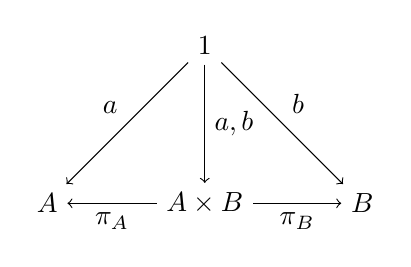
\begin{tikzpicture}[auto]
				\node (a) at (0, 0) {$A$};
				\node (b) at (4, 0) {$B$};
				\node (ab) at (2, 0) {$A\times B$};
				\node (x) at (2, 2) {$1$};
				\draw[->] (ab) to node {$\pi_A$}(a);
				\draw[->] (ab) to node[swap] {$\pi_B$}(b);
				\draw[->] (x) to node[swap] {$\varDelta a$}(a);
				\draw[->] (x) to node {$\varDelta b$}(b);
				\draw[->] (x) to node {$\tuple{\varDelta a,\varDelta b}$}(ab);
			\end{tikzpicture}
		\end{center}
	\end{proof}
	\begin{proof}[$\Longleftarrow$]
		直積集合の定義より、任意の元$a$、$b$に対して順序対$\tuple{a,b}$が存在し、順序対ではない元や重複する元を含まない。すなわち、順序対$\tuple{a,b}$は要素$a,b$に対して一意に存在する。

		これによって写像$\mor{f}{X}{A}$と写像$\mor{g}{X}{B}$の写像の対$\tuple{f,g}$を$X$の任意の要素$x$に対して\[\tuple{f,g}(x)=\tuple{f(x),g(x)}\]と定義することができるようになる。
    
    またここで射影射となる射影写像$\pi_A,\pi_B$を任意の順序対$\tuple{a,b}$において\[\pi_A(\tuple{a,b})=a,\ \pi_B(\tuple{a,b})=b\]と定義して、写像の対が射の対になることを示せば良い。

		\begin{align*}
			(\pi_A\circ\tuple{f,g})(x)&=\pi_A(\tuple{f,g}(x))&\text{(写像の合成の定義)}\\
			&=\pi_A(\tuple{f(x),g(x)})&\text{(写像の対の定義)}\\
			&=f(x)&\text{(元の対の可換性)}\\
			(\pi_B\circ\tuple{f,g})(x)&=\pi_B(\tuple{f,g}(x))&\text{(写像の合成の定義)}\\
			&=\pi_B(\tuple{f(x),g(x)})&\text{(写像の対の定義)}\\
			&=g(x)&\text{(元の対の可換性)}
		\end{align*}
		よって\[\pi_A\circ\tuple{f,g}=f,\ \pi_B\circ\tuple{f,g}=g\]が成り立つから写像の対は射の対としての可換性を満たし、任意の射$f,g$に対して存在することが分かった。
    
		一意性については仮に$\pi_A\circ h=f,\ \pi_B\circ h=g$となる射$\mor{h}{X}{A\times B}$が存在しても、
		$\pi_A(h(x))=f(x),\ \pi_B(h(x))=g(x)$と順序対の一意性より$h(x)=\tuple{f(x),g(x)}$が成り立ち$h=\tuple{f,g}$となる。よって写像$f,g$の写像の対$\tuple{f,g}$は一意に存在する。
	\end{proof}
	